% Software Frontend (HTML/CSS/JS; Vue.js)
% Zuständig: Arthur

\section{Software - Frontend}
\label{sec:software_frontend}
Das Frontend wurde als Webanwendung realisiert,
welche die vom Server gesammelten Daten visualisiert.
%
Dazu zählen z.B. die Daten vom LiDAR-Sensor,
vom Beschleunigungssensor
und die Geschwindigkeit der Roboter,
welche mithilfe der Encoder ausgelesen wird.
%
Um die Aktivitäten der Roboter mitverfolgen zu können,
ohne vor Ort anwesend sein zu müssen,
werden auch die Livestreams von Kameras,
welche auf den Robotern angebracht sind,
angezeigt.

Das Frontend wird mithilfe von Vue.js programmiert.
%
Vue.js ist ein JavaScript-Framework zur Webentwicklung
und bietet verschiedene Möglichkeiten,
Webseiten zu programmieren.
%
Bei Vue.js kann man zwischen der ``Options'' oder
der neueren ``Composition'' API unterscheiden.
%
Die Composition API ist etwas flexibler in der Anwendung,
während die Options API eine klar definierte Struktur verfolgt.
%
Letztlich ist es dem Entwickler überlassen,
je nach seinen Präferenzen zu wählen.
%
Wir verwenden für unsere Anwendung die Composition API,
da diese etwas intuitiver ist
und ``normalem'' JavaScript etwas näher kommt. 
%
Der große Vorteil des Vue.js Frameworks ist,
dass man einzelne Komponenten einer Website
als sogenannte SFC\footnote{Single-File Components}s definiert.
%
Wie der Name schon impliziert ist in diesem SFC alles enthalten,
was diese Komponente braucht: HTML, CSS und Type-/JavaScript.
%
Dadurch wird der Code schön strukturiert und klar aufgeteilt.
%
Des Weiteren können Vue-Komponenten auch
in anderen Komponenten wiederverwendet werden,
was eine schöne Abstrahierung ermöglicht.

\subsection{LiDAR-Karte}
\label{subsec:frontend_lidar_map}
Die LiDAR-Karte wird mithilfe von Vue.js auf dem Frontend,
der Webseite,
generiert und soll Hindernisse wie Wände,
Säulen oder auch Menschen mit farbigen Punkten anzeigen.
%
Hierbei gibt es aber keine Klassifikation des Hindernistyps,
abgesehen von der Erkennung von Tamerlan und Bambi.
%
Neben der verschiedenen Hindernisse,
die auf der Karte einzusehen sind,
sollen auch die Position der Roboter markiert werden.

\begin{figure}[H]
    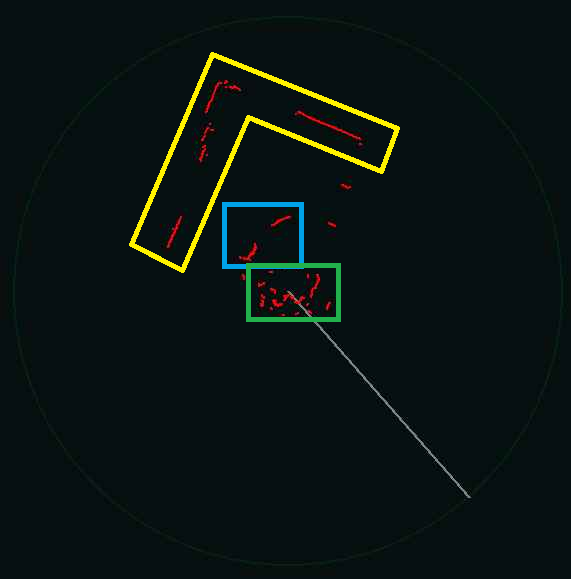
\includegraphics[width=0.4\textwidth, center]{img/LiDARMessungZeichnung_alt.png}
    \caption{LiDAR-Messung}
    \label{fig:LiDAR-Messung}
\end{figure}

Das Bild zeigt die generierte Punktwolke des LiDAR-Sensors.
%
Die Punktwolke zeigt ideal die Funktionsweise des LiDARs
und ist leicht zu interpretieren.
%
Die unterschiedlichen Laserimpulse,
welche gesendet werden,
reflektieren an der Oberfläche und werden gemessen.
% TODO @Arthur was hast du da gemeint???
Nicht nur ist die Entfernung, sondern auch die Tiefenwahrnehmung somit feststellbar.

Zur einfacheren Interpretation des Beispiels
wurden von Herrn Burjak Bereiche eingezeichnet:
%
Der grüne Bereich zeigt Objekte,
welche unmittelbar vor dem LiDAR standen.
%
In dem Fall waren es Büromaterialien wie etwa Kugelschreiber, Hefte, etc.
%
Blau markiert ist eine Person (links),
die ungefähr in 2.5 m Entfernung vom Sensor
neben einem Sessel (rechts) steht.
%
Im gelbem ``L'' kann man die Wände bzw. Bücherregale erkennen,
welche den Testraum abgegrenzt haben.
Die beiden großen Lücken im gelbem Bereich wurden
durch die Hindernisse im blauem Bereich verursacht,
an denen der Laser bereits schon frühzeitig abgeprallt ist.
%
Die beiden nicht markierten Punkte-``Cluster'' stellen Dachstützen dar.


\subsection{Fernüberwachung per Kamera}
\label{subsec:frontend_cam_stream}
Auf allen drei Robotern befinden sich fest montierte
\texttt{ESP32-CAM}-Kameramodule zur Überwachung,
welche dem Frontend via MJPEG ein Live-Bild bereitstellen.
%
Die Kameras dienen vor allem der Überwachung der Roboter und sollen der Gruppe nur helfen,
mögliche Probleme (z.B. Stiegen) rasch zu identifizieren,
um die Sicherheit der Roboter zu gewährleisten.
%
Eingriffe erfolgen nur falls die Roboter nicht selbstständig erfolgreich die Gefahrensituation vermeiden.
%
Sollte ein Fehler bei der autonomen Steuerung von einem der Roboter aufgetreten sein,
helfen uns die Kameras zusätzlich bei der manuellen Fernsteuerung.
%
So können wir mithilfe der Fernsteuerung (Siehe Abschnitt \ref{subsec:frontend_control}) probieren,
die Roboter z.B. aus einer Gefahrenzone zu entfernen.

\subsection{Fernsteuerung}
\label{subsec:frontend_control}
Das Konzept der Fernsteuerung wurde aus den Prototypen der Projektwoche aus dem Jahr 2023/2024 übernommen.
%
Diese hatten eine Fernsteuerungsfunktion,
welche hier in der Diplomarbeit nur zu Testzwecken oder in Gefahrensituationen verwendet wird.  

\subsection{Anzeigen der Sensordaten}
\label{subsec:frontend_sensors}
Die Sensordaten werden alle auf dem Frontend dargestellt und stetig aktualisiert.
%
Jeder Tumbller-Roboter ist ab Werk mit Beschleunigungssensoren und Drehgebern ausgerüstet,
welche wir gleich für unsere Zwecke wiederverwendet haben.
%
Als Modifikationen haben wir jedem Roboter ein Kompass-Modul
und Guide zusätzlich noch den LiDAR installiert.
%
Der LiDAR erstellt eine Karte in Form einer Punktwolke,
um eventuelle Hindernisse erkennen zu können.
%
Für mehr Informationen zum LiDAR-Sensor siehe Abschnitt \ref{subsec:frontend_lidar_map}.

%TODO BILD ÄNDERN
\begin{figure}[H]
    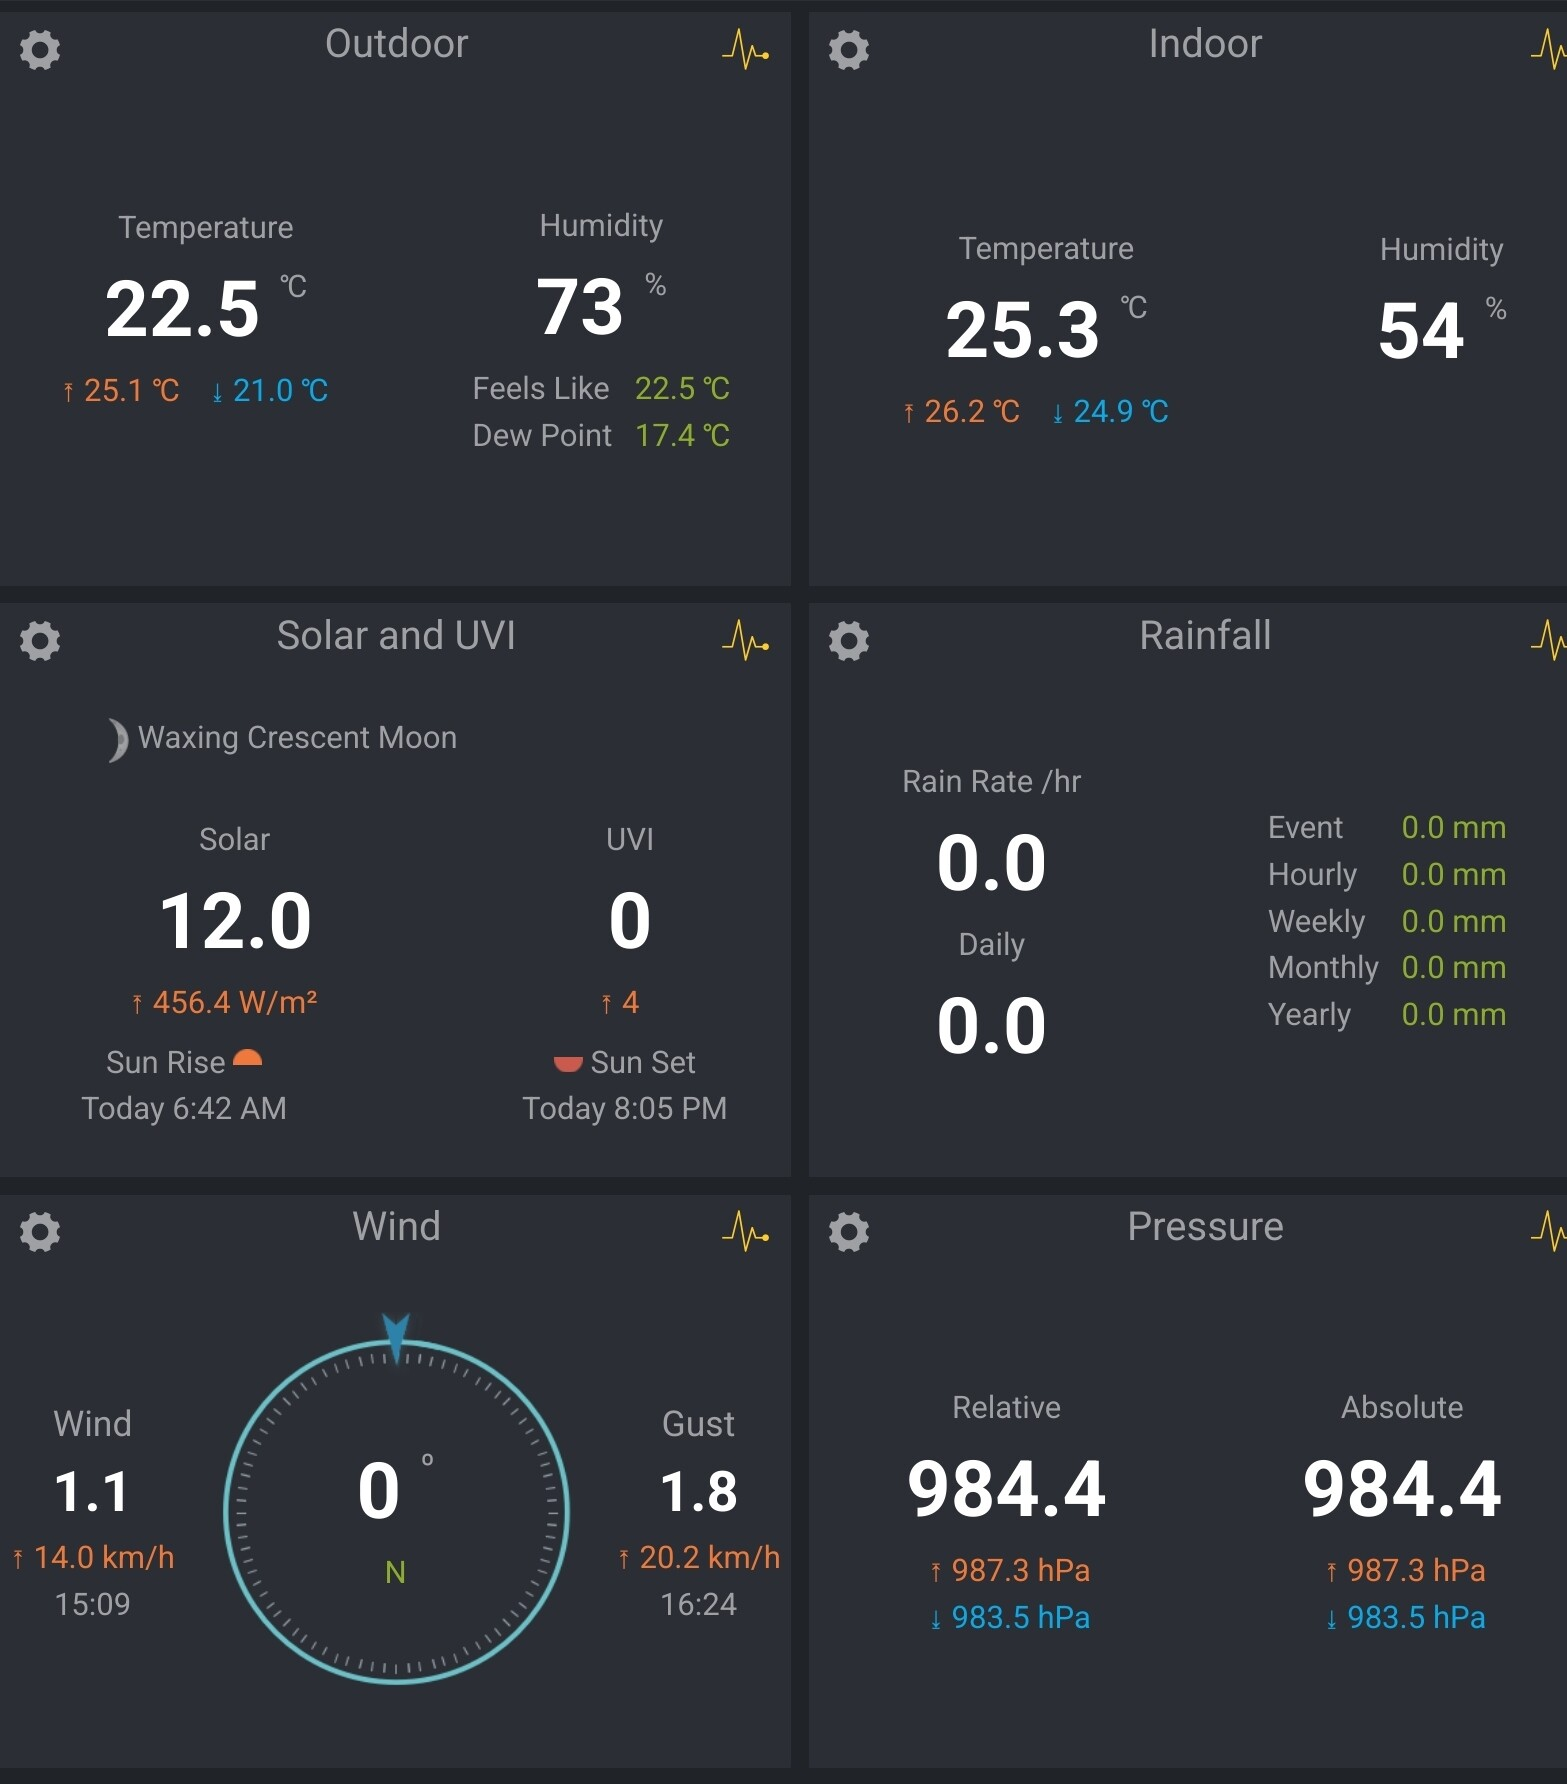
\includegraphics[width=0.4\textwidth, center]{img/Sensor_Anzeige_LOESCHEN.png}
    \caption{Anzeige der Sensordaten}
    \label{fig:Sensordaten}
\end{figure}

Die Werte der Beschleunigungssensoren werden,
neben der einfachen Anzeige als Dezimalzahl,
zusätzlich in Graphen abhängig von der Zeit angezeigt,
um die aktuellen Werte mit der Vergangenheit vergleichen zu können.

Die Kompasse zeigen die aktuelle Fahrtrichtung der Roboter an.
% TODO @Arthur wie soll die Nadel auf einem vertikalen Bildschirm eine horizontale Richtung anzeigen?
%  Woher wissen wir, in welche Richtung der Bildschirm zeigt?
Geplant ist ein ``realer'' 2D-Kompass,
wobei jedoch die Nadel die Fahrtrichtung anzeigt,
statt wie gewohnt den Norden.